\chapterimage{orange2.jpg}
\chapterspaceabove{6.75cm} 
\chapterspacebelow{7.25cm} 
\chapter{Preliminary Number Theory and Cryptography}
%intro
In this chapter, we will look into one of the most exciting part of mathematics, and it is also a
crucial cornerstone for computer science. The inception of number theory can be traced back to ancient civilizations, but it began to emerge as a distinct mathematical discipline with the work of the Greek mathematician Euclid. His monumental work, "Elements," laid the groundwork for the study of prime numbers and proved fundamental theorems, such as the infinitude of primes, which are still central to number theory today. The nature of whole numbers, especially the intriguing properties of prime numbers—the building blocks of all natural numbers—has fascinated mathematicians for centuries. Over time, the field has expanded to include a rich array of topics such as the distribution of primes, the solutions of Diophantine equations, modular arithmetic, and the exploration of number-theoretic functions like the Riemann zeta function. Number theory's initial focus on prime numbers and divisibility has blossomed into a diverse and vibrant branch of mathematics, with applications ranging from cryptography to the theory of chaos.

\section{Divisibility and Modular Arithmetic}
We start with the divisibility of number, as it is the basis of many further topics.
Divisibility serves as the cornerstone of number theory due to several pivotal reasons. It is the bedrock upon which the Fundamental Theorem of Arithmetic stands, declaring that each integer greater than 1 is uniquely decomposable into a product of prime numbers. These primes are the elemental units, akin to atoms in chemistry, from which all other numbers are constructed. The concepts of greatest common divisors and least common multiples emerge from divisibility, forming the basis of crucial algebraic structures such as rings and fields, and thereby extending number theory into algebraic realms. Furthermore, the pursuit of integer solutions to equations, known as Diophantine analysis, is deeply reliant on principles of divisibility. In the modern context, divisibility underpins cryptographic systems, leveraging the challenging task of prime factorization to secure digital communication. Moreover, divisibility naturally extends to modular arithmetic, enriching number theory with the study of congruences, which has profound implications across mathematics and its myriad applications. Therefore, the study of divisibility is not just foundational but also a connective thread that weaves through the entire fabric of number theory.

\subsection{Division and Divisibility}
To figure out problems related to \textbf{Divisibility}, we must figure out the definition and properties
of \textbf{Division}. We were taught in the primary school that a division is an operation  that
divides a number to a certain part. For instance, $6\div2=3$, and $6\div4=1.5$. Sometimes, the
division produce an integer as result, while sometimes not. We define division as follows:
    \begin{definition}[Division]
        The division of a number \( a \) by a non-zero number \( b \) is denoted by \( a \div b \) or \( \frac{a}{b} \), and it gives the quotient \( q \) and possibly a remainder \( r \). The operation can be written as:
        \[
        a = b \times q + r
        \]
        where \( 0 \leq r < b \) and \(q \in \mathbb{Z}\).
    \end{definition}
    In $6\div2=3$, clearly we have $6=2\times3+0$, with $r=0$, $q=3$. But how could we explain
    $6\div4=1.5$? The quotient is a decimal instead of an integer. Fundamentally, we cannot separate
    the number 6 in to 4 parts to be represented as integer. In this case the division can be represented
    as $6 = 4\times0+6$, meaning $q=0$ and $r=6$. Actually, $6\div4=1.5$ is not defined as only
    division, but \textbf{True Division}.
    \begin{definition}[True Division]
        True division is concerned with the quotient including the remainder as a fractional part. In true division, when \( a \) is divided by \( b \), the quotient \( q \) is a real number that can be represented as:
        \[
        q = \frac{a}{b}
        \]
    \end{definition}
    You may find that true division doesn't have a remainder. This is just because the purpose of 
    these two operations are different, as true division only focus on the scale of each part of
    $a$, but division involves the divisibility and remainder, which will be discussed further
    in this chapter.

    Now that we have defined division and true division, you may understand the following definition
    of divisibility easier.
    \begin{definition}[Divisibility]
        If $a$ and $b$ are integers with $a \neq 0$, we say that $a$ divides $b$ if there is an integer $c$ such that $b = a\times c$ (or equivalently, if $b$ a is an integer). When $a$ divides $b$ we say that $a$ is a factor or divisor of $b$, and that $b$ is a multiple of $a$. The notation a $\mid$ b denotes that $a$ divides $b$. We write $a \nmid b$ when $a$ does not divide $b$
    \end{definition}
    For example, we have $4\mid 20$, because $20\div4$ gives an integer, however, $4\nmid 21$, as the answer
    cannot be represented as integer. Besides, we have:
    \begin{equation}
        a\mid b \iff \exists c(ac=b).
    \end{equation}

    \begin{problem}
        Let \( n \) and \( d \) be positive integers. How many positive integers not exceeding \( n \) are divisible by \( d \)?
    \end{problem}
    \textbf{Solution:} The positive integers divisible by \( d \) are all the integers of the form \( dk \), where \( k \) is a positive integer. Hence, the number of positive integers divisible by \( d \) that do not exceed \( n \) equals the number of integers \( k \) with \( 0 < dk \leq n \), or with \( 0 < k \leq \frac{n}{d} \). Therefore, there are \( \left\lfloor \frac{n}{d} \right\rfloor \) positive integers not exceeding \( n \) that are divisible by \( d \).

    Divisibility holds the following properties, which could be proven directly.
    \begin{theorem}[Properties of Divisibility] \label{Properties of Divisibility}
        Let $a$, $b$, and $c$ be integers, where $a\neq 0$, then:
        \begin{enumerate}
            \item if $a \mid b$ and $a \mid c$, then $a \mid (b+c)$
            \item if $a \mid b$ then $a \mid bc$ for all integers $c$
            \item if $a \mid b$ and $b\mid c$, then $a \mid c$
        \end{enumerate}
    \end{theorem}
    \begin{proof}
        Since \( a \mid b \) and \( a \mid c \), there exist integers \( m \) and \( n \) such that \( b = am \) and \( c = an \). Therefore, \( b+c = am + an = a(m+n) \), and since \( m+n \) is an integer, it follows that \( a \mid (b+c) \).
        
        Given \( a \mid b \), there exists an integer \( k \) such that \( b = ak \). For any integer \( c \), \( bc = a(kc) \). Since \( kc \) is an integer (because the product of two integers is an integer), \( a \mid bc \).
        
        If \( a \mid b \) and \( b \mid c \), then there exist integers \( p \) and \( q \) such that \( b = ap \) and \( c = bq \). Substituting the expression for \( b \) into the equation for \( c \) gives \( c = (ap)q = a(pq) \). Since \( pq \) is an integer, \( a \mid c \).
    \end{proof}
    With this we have the following conclusion.
    \begin{corollary}\label{div1}
        if $a$, $b$, and $c$ are integers, where $a\neq 0$, such that $a\mid b$ and $a\mid c$, then $a\mid mb + nc$ whenever $m$ and $n$ are integers.
    \end{corollary}
    This could be proven in direct proof, which you will finish in the exercise.

    \subsection{Modular Arithmetic}
    In this section, we will focus on the remainder of division, as well as modular arithmetic.
    In the definition of division, we involved $q$ and $r$, which denotes the quotient and
    the remainder of the operation. We use the following notations to denote each of both.
    \begin{notation}[div and mod]
        For $a$, $b\in \mathbb{R}$.
        $a = b\times q + r$    
        $$q = a\ \text{\textbf{div}}\ b$$
        $$r = a\ \text{\textbf{mod}}\ b$$
    \end{notation}
    Besides, when $a$ is an integer and $b$ is a positive integer, we have $a\ \text{\textbf{div}}\ b = \left \lfloor  a/b \right \rfloor$.
    \begin{example}
        What are the quotient and remainder when 93 is divided by 9?
    \end{example}
    \textbf{Solution:} $93 = 9\times 10 + 3$. $q = 10$, $r = 3$.

    The quotient is $93\ \textbf{div}\ 9 = 10 = \lfloor93/9\rfloor = \lfloor10.3333\dots \rfloor = 10$

    The remainder is $93\ \textbf{mod}\ 9 = 3 = 93 - 90$
    \begin{problem}
        Is it possible for the remainder to be negative?
    \end{problem}
    In most cases, we see positive remainder, as if it were the only possibility. However, we can
    refute this using one example.
    \begin{example}
        What are the quotient and remainder when -93 is divided by 9?
    \end{example}
    \textbf{Solution:} $-93 = 9\times (-11) + 6$. $q = -11$, $r = 6$.
    
    Remember that we must make sure $r\geq0$ as we defined earlier, even though $-93 = 9\times(-10) - 3$.
    But remainder could be positive in other division algorithm, which we will discuss in the exercise.

    We have already introduced the notation $ a\ \textbf{mod}\ m $ to represent the remainder when an integer
    $a$ is divided by the positive integer $m$. We now introduce a different, but related, notation
    that indicates that two integers have the same remainder when they are divided by the positive
    integer $m$. But why we need to find and study the numbers with the same remainder by dividing 
    the same positive integer? Studying numbers that yield the same remainder when divided by a given positive integer is a
    fundamental part of number theory; later you will understand why say so.
    \begin{definition}
        If $a$ and $b$ are integers and $m$ is a positive integer, then $a$ is \textbf{congruent} 
        to $b$ \textbf{modulo} $m$ if $m$ divides $a - b$. 
        We use the notation $a \equiv b (\bmod m)$ to indicate that $a$ is congruent to $b$ modulo 
        $m$. We say that $a \equiv b (\bmod m)$ is a congruence and that $m$ is its modulus 
        (plural moduli). If $a$ and $b$ are not congruent modulo $m$, we write $a \not\equiv b (\bmod m)$.
    \end{definition}
    Do note that mod and \textbf{mod} are different notations. The first represents a relation on the set of integers, whereas the
    second represents a function. However, they are still related.
    \begin{theorem}
        Let $a$ and $b$ be integers, and let $m$ be a positive integer. $a \equiv b (\bmod \  m)$ if and only if $a\ \textbf{mod}\ m$ = $b\ \textbf{mod}\ m$.
    \end{theorem}
    \begin{proof}
        First, suppose \( a \equiv b \pmod{m} \). By definition of congruence modulo \( m \), \( m \) divides \( a - b \), which means there exists some integer \( k \) such that \( a - b = km \).

        Dividing \( a \) and \( b \) by \( m \), they both leave the same remainder \( r \), since \( a = q_1m + r \) and \( b = q_2m + r \) for some integers \( q_1 \) and \( q_2 \). The remainder \( r \) in both cases is the same because the difference \( a - b \) is a multiple of \( m \), which does not affect the remainder.

        Conversely, if \( a \mod m = b \mod m \), then both \( a \) and \( b \) leave the same remainder when divided by \( m \). Denote this common remainder as \( r \).

        We can write \( a = q_1m + r \) and \( b = q_2m + r \) for some integers \( q_1 \) and \( q_2 \). Subtracting these two equations, we get \( a - b = (q_1 - q_2)m \), which shows that \( a - b \) is a multiple of \( m \).

        Therefore, \( m \) divides \( a - b \), and by definition of congruence modulo \( m \), we have \( a \equiv b \pmod{m} \).

        This completes the proof.
    \end{proof}
    \begin{remark}
        Remember, when we say if and only if, we need proof from each of the both statements to the other.
    \end{remark}
    \begin{theorem}\label{mod2}
        Let $m$ be a positive integer. The integers $a$ and $b$ are congruent modulo $m$ if and only if there is an integer $k$ such that $a = b + km$.
    \end{theorem}
    The proof is similar and not complex, try to prove it in the exercise.







    \subsection{Exercises}
    \begin{exercise}
        Prove corollary \ref{div1} that if $a$, $b$, and $c$ are integers, where $a\neq 0$, such that $a\mid b$ and $a\mid c$, then $a\mid mb + nc$ whenever $m$ and $n$ are integers.
    \end{exercise}
    \begin{proof}
        By theorem \ref{Properties of Divisibility}, $a\mid b$ and $a\mid c$ gives us $a\mid mb$
        and $a\mid nc$ (property 2). Hence, $a\mid (mb+nc)$ (property 1). This completes the proof.
    \end{proof}
    
    \begin{exercise}
        floored division he truncated division
    \end{exercise}

    \begin{exercise}
        Prove theorem \ref{mod2}, you may use other theorems or corollary in this chapter.
    \end{exercise}
    \begin{proof}
        If $a \equiv b (\bmod \ m)$, that means we have $m\mid(a-b)$. There must be a integer $k$, such that $a = b + km$ (theorem \ref{mod2}). Conversely, if we have a integer $k$, such that $a = b+km$, we have $km = a-b$. Hence, $m\mid(a-b)$, $a \equiv b (\bmod \ m)$.
    \end{proof}
    \begin{exercise}
        show that for integer $\displaystyle a,\ b,\ c\ \in \mathbb{Z}^{+}$, $\displaystyle a,c\neq 0$ and $\displaystyle ac\mid bc,$then $\displaystyle a\mid b$.
    \end{exercise}
    \begin{proof}
        $\displaystyle ac\mid bc$ means that $\displaystyle bc=k( ac)$ for some integer $\displaystyle k$, so we have $\displaystyle b=ka$, this means $\displaystyle a\mid b$.
    \end{proof}
    \begin{exercise}
        Prove that if $\displaystyle a$ and $\displaystyle b$ are integers and $\displaystyle a$ divides $\displaystyle b$, then $\displaystyle a$ is odd or $\displaystyle b$ is even.
    \end{exercise}
    \begin{proof}
        We could try proof by contrapositive. Suppose for $\displaystyle a$ is even and $\displaystyle b$ is odd, 
        $\displaystyle a,b\in \mathbb{Z} ,\ a\mid b$. Then $\displaystyle b=ka$ for some integer $\displaystyle k$. 
        Make $\displaystyle a=2n,\ b=2n+1,\ n\in \mathbb{Z}$, then there should be $\displaystyle 2n+1=2kn$. 
        However, in this case we have $\displaystyle k=\frac{2n+1}{2n}$, meaning that $\displaystyle k$ is not an 
        integer, which contradict the assumption. This completes the proof.
    \end{proof}
    \begin{exercise}
        Prove that if $a$ is a positive integer, then $4\nmid (a^2+2)$.
    \end{exercise}
    \begin{proof}
        Consider any positive integer $a$. We know that $a$ can be expressed in one of the following forms where $n$ is an integer:
        \begin{itemize}
            \item $a = 4n$
            \item $a = 4n + 1$
            \item $a = 4n + 2$
            \item $a = 4n + 3$
        \end{itemize}
        Now, we examine $a^2$ modulo 4 for each case:
        \begin{align*}
            (4n)^2 &= 16n^2 = 4 \cdot 4n^2 \equiv 0 \pmod{4}, \\
            (4n + 1)^2 &= 16n^2 + 8n + 1 = 4(4n^2 + 2n) + 1 \equiv 1 \pmod{4}, \\
            (4n + 2)^2 &= 16n^2 + 16n + 4 = 4(4n^2 + 4n + 1) \equiv 0 \pmod{4}, \\
            (4n + 3)^2 &= 16n^2 + 24n + 9 = 4(4n^2 + 6n + 2) + 1 \equiv 1 \pmod{4}.
        \end{align*}
        Adding 2 to $a^2$ in each case yields:
        \begin{align*}
            a^2 + 2 &\equiv 2 \pmod{4} \quad \text{if } a^2 \equiv 0 \pmod{4}, \\
            a^2 + 2 &\equiv 3 \pmod{4} \quad \text{if } a^2 \equiv 1 \pmod{4}.
        \end{align*}
        In both cases, $a^2 + 2$ does not yield a remainder of $0$ modulo $4$. Thus, it cannot be divisible by $4$.

        Therefore, we have proven that for any positive integer $a$, the expression $a^2 + 2$ is not divisible by $4$.
    \end{proof}


    \section{Number Representations and Algorithms}
    In everyday life, we use decimal notation to express integers. Though this is not
    for all cases, as we are using a 60 base system for time. However, in computer science, binary, octal, and hexadecimal
    systems are widely used for number representation. The reason is that binary system consist of 
    only 0 and 1, as we have mentioned in Boolean algebra, this system is perfect for logic operations
    in side the computer. What's more, 0 and 1 could be easily represented by the on and off of tiny
    switches in the integrated circuits. This chapter looks into the representation of number
    in different bases and their relationship, with a tress on binary representation that computer
    system uses. Meanwhile, we will go through algorithm of some operations between number, and
    analyze them accordingly.
    \subsection{Representations of Numbers and Base Conversion}
    In whichever base, a number could be expressed using the exponent of the base.
    \begin{theorem}[Representation of Number]
		Let $b$ be an integer greater than 1. Then if $n$ is a positive integer, it can be expressed uniquely 
		in the form:\\
		$n=a_{k} b^{k}+a_{k-1} b^{k-1}+\cdots+a_{1} b+a_{0}$\\
		where $k$ is a nonnegative integer, $a_0, a_1,\cdots, a_k$ are negative integers less than b, and $a_k \neq 0$
	\end{theorem}
    For example, 1024 could be interpreted as $1024 = 1\times10^3+\times10^2+2\times10^1+4\times10^0$.
    Besides, the base of number constraints the possible numbers to be used on the bits. For example,
    under decimal system, we cannot take 10 as one digit, instead it is a number with two digits 1 and 0,
    because for bits under decimal system, the maximum only goes to 9. Therefore, you could take it as
    a fact that for a system of base $b$, the biggest value for one bit is $b-1$. Similarly, we see
    only 0 and 1 in binary, 1-7 in ocatl, 1-15 in hexadecimal expression.

    To indicate the base of a number, we use the following subscript.
    \begin{notation}[$xxxx_b$]
        We use $_b$ to show the base of a number, where $b$ is the base number.
    \end{notation}

    The other important fact is that numbers are just numbers, base is only the way we gauge them.
    However you change $121_{10}$, to whatever base, it is still 121 in decimal, but just expressed 
    in a different way.
    \subsubsection*{Binary, Octal, and Hexadecimal Expression}
    In \textbf{binary expansion}, the base on any integer is 2, that is to say, the number in each digit is either 0 or 1.
We can expand binary integer in the same ways as mentioned in last section.

\begin{example}
	What is the decimal expansion of the integer that has $(101011111)_2$ as its binary expansion?

		$(101011111)_2$ has nine digits, so we have:\\
		$(101011111)_2$ = $1\times 2^9 + 1\times 2^7+1\times 2^5+1\times 2^4+1\times 2^3+1\times 2^2+1\times 2^1+1\times 2^0 = 351$

\end{example}
Decimal expansion of octal expansions could be calculated in the same way as the binary expansion. However, 
Sixteen different digits are required for hexadecimal expansions. Usually, the hexadecimal digits used are 
0, 1, 2, 3, 4, 5, 6, 7, 8, 9, A, B, C, D, E, and F, where the letters A through F represent the digits 
corresponding to the numbers 10 through 15 (in decimal notation). 
\begin{example}
	What is the decimal expansion of the number with hexadecimal expansion $(2AE0B)_{16}$?
\end{example}
In hexadecimal cases, the only difference is that capital latters are used to represent two-digit number in
		one digit. We still have:\\
		$(2AE0B)_{16}$ = $2\times 16^4 + 10\times 16^3 + 14\times 16^2 + 0 \times 16^1 + 11 \times 16^0=175627$

        \textbf{NOTICE: } Each hexadecimal digit can be represented using four bits. For instance, 
we see that $(1110 0101)_2$ = $(E5)_{16}$ because $(1110)_2$ = $(E)_{16}$ and $(0101)_2 = (5)_{16}$. Bytes, which are bit strings 
of length eight, can be represented by two hexadecimal digits.

    \subsection{Base Conversion}
    \subsubsection*{Base conversion of Integer}
    Now we have learned how to express numbers in different base systems, but is there any way to
    convert them from one base to the other? You may have realized that a general solution is to
    convert the number back to decimal form, and then to the target base. Yes, it works, but can we
    make it better? One way to this is to use the general base conversion algorithm.
    The most common algorithm to constructing the base $b$ expansion of an integer n is as follows:\\
First, divide $n$ by $b$ to obtain a quotient and remainder, that is: \\
\begin{center}
	$\displaystyle n\ =\ bq_{0} \ +\ a_{0} \ \ \ \ \ \ \ \ \ \ \ \ \ \ \ \ \ \ \ \ \ ( 0\ \leq \ a_{0} \ < \ b)$
\end{center}
The remainder, $a_0$, is the rightmost digit in the base b expansion of $n$. Next, divide $q_0$ by $b$ toobtain:\\
\begin{center}
	$\displaystyle q_0\ =\ bq_{1} \ +\ a_{1} \ \ \ \ \ \ \ \ \ \ \ \ \ \ \ \ \ \ \ \ \ ( 0\ \leq \ a_{1} \ < \ b)$
\end{center}
We see that $a_1$ is the second digit from the right in the base b expansion of n. Then, we just continue this process
until we obtain a quotient equal to zero. This algorithm produces the base $b$ digits of $n$ from the right to the left.

\begin{example}
	Find the hexadecimal expansion of $(177130)_{10}$.
		\begin{center}
		$177130 = 16 \cdot 11070 + 10$\\
		$11070 = 16 \cdot 691 + 14$\\
		$691 = 16 \cdot 43 + 3$\\
		$43 = 16 \cdot 2 + 11$\\
		$2 = 16 \cdot 0 + 2 $\\
		\end{center}
		Therefore, $(177130)_{10} = (2B3EA)_{16}$
\end{example}
    This method is equivalent to the following pseudocode.
    \begin{algorithm}
        \caption{Base conversion of an integer $n$ to base $b$}
        \begin{algorithmic}[H]
        \Require{An integer $n$ and a base $b$ to convert to}
        \Ensure{The base $b$ expansion of $n$}
        \Function{ConvertToBase}{$n, b$}
            \State $digits \gets$ empty list
            \While{$n > 0$}
                \State $remainder \gets n \bmod b$
                \State Append $remainder$ to $digits$
                \State $n \gets \left\lfloor n / b \right\rfloor$
            \EndWhile
            \State $digits \gets$ reverse $digits$
            \State \textbf{return} $digits$
        \EndFunction
        \end{algorithmic}
        \end{algorithm}
    \subsubsection*{Base Conversion of Float}
    The previous algorithm only deals with integers, so we need a different approach for decimals.
    The algorithm for converting a floating-point number from base 10 to base $b$ is given as follows:

\begin{algorithm}
\caption{Convert a floating-point number to a different base}
\begin{algorithmic}[1]
\Function{ConvertFloatToBase}{$number$, $targetBase$}
    \State $integerPart \gets \lfloor number \rfloor$
    \State $fractionalPart \gets number - integerPart$
    \State $baseInteger \gets \Call{ConvertIntegerToBase}{integerPart, targetBase}$
    \State $baseFraction \gets ``"$
    \While{$fractionalPart > 0$ \textbf{and} length of $baseFraction$ is less than limit}
        \State $fractionalPart \gets fractionalPart \times targetBase$
        \State $baseFraction \gets baseFraction + \lfloor fractionalPart \rfloor$
        \State $fractionalPart \gets fractionalPart - \lfloor fractionalPart \rfloor$
    \EndWhile
    \State \Return $baseInteger + ``." + baseFraction$
\EndFunction
\end{algorithmic}
\end{algorithm}

\begin{example}
Convert the floating-point number 12.375 from base 10 to base 2.
\begin{itemize}
\item Integer part: 12 in base 10 is 1100 in base 2.
\item Fractional part: 0.375 in base 10 to base 2.
\begin{align*}
0.375 \times 2 &= 0.75 \rightarrow \text{integer part is 0} \\
0.75 \times 2 &= 1.5 \rightarrow \text{integer part is 1} \\
0.5 \times 2 &= 1 \rightarrow \text{integer part is 1} \\
\end{align*}
\item The fractional part in base 2 is .011.
\end{itemize}

Therefore, $12.375_{10}$ is $1100.011_{2}$.
\end{example}
Also, when a number consist of both integer and decimal parts, we just deal with them separately
and them put them back together later. You will see these exercises in the problem set.

\subsubsection*{Base Conversion between Binary, Octal, and Hexadecimal number}
The base conversion between Binary, Octal and Hexadecimal numbers are much easier.
\begin{figure}[H]
	\centering
	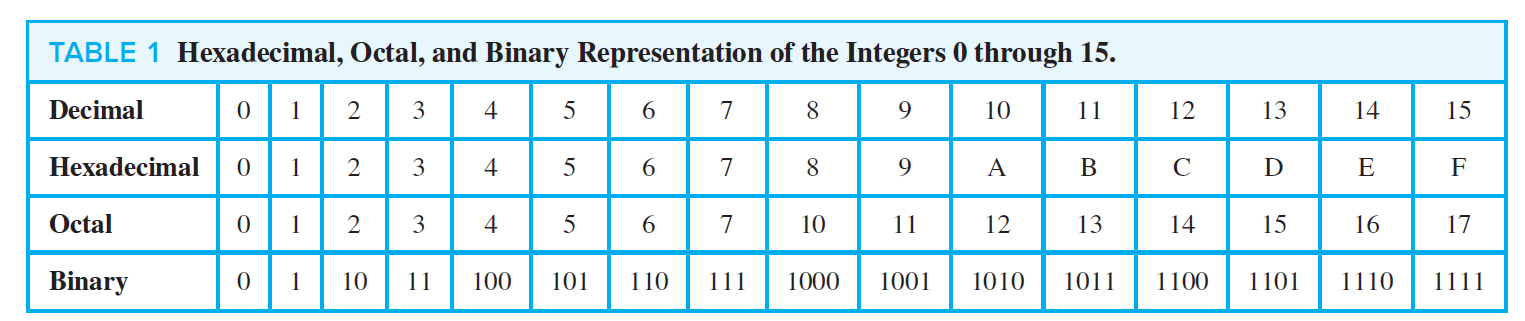
\includegraphics[width=1\linewidth]{converttab.png}
    \caption{Binary, Octal and Hexadecimal Representation}
\end{figure}
The conversion between binary, octal, and hexadecimal systems is straightforward because the bases of these systems (2 for binary, 8 for octal, and 16 for hexadecimal) are related by powers of 2. Specifically:
\begin{itemize}
    \item Octal digits correspond to three binary digits since \(8 = 2^3\). Each octal digit can be directly mapped to a unique combination of three binary bits.
    \item Hexadecimal digits correspond to four binary digits since \(16 = 2^4\). Each hexadecimal digit can be directly mapped to a unique combination of four binary bits.
\end{itemize}
This relationship allows for simple grouping of binary bits into sets of three or four to convert 
to octal or hexadecimal, respectively, without any complex calculation or division. 
\begin{example}
	Find the octal and hexadecimal expansions of $(11\ 1110\ 1011\  1100)_2$ and the binary expansions of $(765)_{8}$ and $(A8D)_{16}$.
\end{example}
\textbf{Solution:} To convert $(11\ 1110\ 1011\  1100)_2$ into octal notation we group the binary digits
into blocks of three, adding initial zeros at the start of the leftmost block if necessary.
These blocks, from left to right, are 011, 111, 010, 111, and 100, corresponding to 3, 7, 2, 7, and 4 respectively. Consequently, we get $(11\ 1110\ 1011\  1100)_2 = (37274)_8$
\par We do the hexadecimal convention in the same way. These blocks, from left to right, are 0011,
1110, 1011, and 1100, corresponding to the hexadecimal digits 3, E, B, and C, respectively. Consequently, $(11\ 1110\ 1011\  1100)_2 = (3EBC)_{16}$
\par \textbf{NOTE: } The conversion could be done inversely in the same way. If the number of bit is not the multiple of 4 when you are converting between 2 and 16 base
number, fill those missing digits/bits with 0.

Whether you noticed or that the base conversion, essentially, is about division and modular arithmetic
that we just learned? The general base conversion algorithm could be simplified to the following algorithm,
where $n$ denotes the number to be converted and $b$ is the target base.
\begin{algorithm}
    \caption{Constructing Base \( b \) Expansions}
    \begin{algorithmic}[1]
    \Procedure{base \( b \) expansion}{$n, b$: positive integers with $b > 1$}
    \State $q \gets n$
    \State $k \gets 0$
    \While{$q \neq 0$}
    \State $a_k \gets q \mod b$
    \State $q \gets \lfloor q / b \rfloor$
    \State $k \gets k + 1$
    \EndWhile
    \State \textbf{return} $(a_{k-1}, \ldots, a_1, a_0)$ \Comment{The base \( b \) expansion of \( n \)}
    \EndProcedure
    \end{algorithmic}
    \end{algorithm}
    \subsection{Operation Algorithms of Number}
        
    \subsubsection*{Addition Algorithm}

    \subsubsection*{Multiplication Algorithm}

    \subsubsection*{Algorithm for Div and Mod}

    \subsection{Modular Exponentiation}

    \subsection{Exercises}


    \section{Primes and Greatest Common Divisors}

    \subsection{Primes and Trial Division}

    \subsection{Manipulation of Primes}

    \subsection{Greatest Common Divisors and Least Common Multiples}

    \subsubsection*{The Euclidean Algorithm}

    \subsection{Greatest Common Divisors as Linear Combinations}
